\section{Плоская электромагнитная волна. Поляризация.}

\subsection*{Плоская электромагнитная волна}

\[
\begin{aligned}
    (1)
    \begin{cases}
        \vec{E}=\vec{E}_0e^{i\varphi} \\
        \vec{H}=\vec{H}_0e^{i\varphi} 
    \end{cases}
    \text{ , где } \varphi=\varphi_0+\vec{k}\vec{r}-\omega t 
    \Leftrightarrow
    \begin{cases}
        \vec{E}=\vec{E}_0\cos\varphi \\
        vec{H}=\vec{H}_0\cos\varphi
    \end{cases}
\end{aligned}
\]

\[
\boxed{
    \begin{aligned}
        &\frac{\omega}{k}=\frac{c}{n} \text{ , где } n=\sqrt{\varepsilon\mu} \\
        & \text{Рис.1: }[\vec{E}_0,\vec{H}_0,\vec{k}]-\text{образют правую тройку}
    \end{aligned}
}
\]

При таких условиях и только при них плоская электромагнитная волна удовлетворяет всем условиям Максвелла в среде \( \varepsilon,\mu \) без зарядов и токов.

Плоская электромагнитная волна- не единственное решение уравенения Максвелла в среде \( \varepsilon,\mu \) без зарядов и токов.

Поскольку уравенения Максвелла линейны, суперпозиция плоских волн с разными параметрами, удовлетворяет условиям (2) тоже является решением.

\textit{Фронт волны}- геометрическое место точек одинаковой фазы в фиксированный момент времени. 

Есть свобода выбрать \( \vec{k}, \vec{E}_0 \)

\begin{minipage}[c]{0.2\textwidth} % Левая часть: изображение
    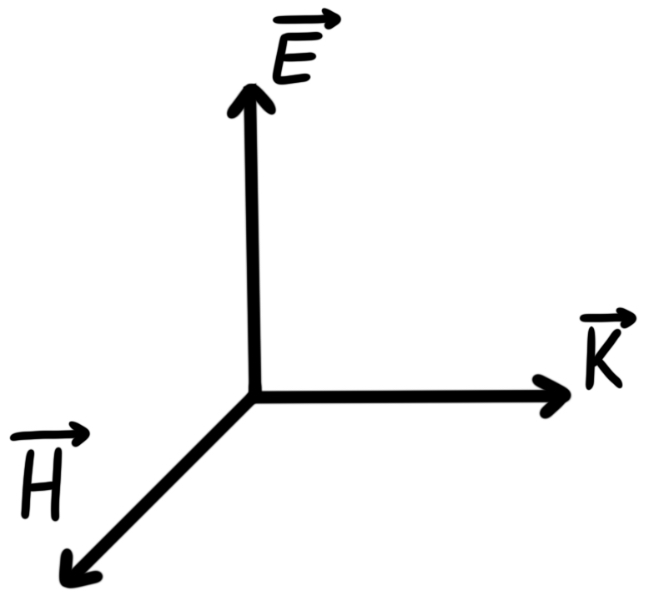
\includegraphics[width=\textwidth]{im/98.png}% Ваше изображение
\end{minipage}%
\hfill
\begin{minipage}[c]{0.6\textwidth} % Правая часть: текст
    \[
    \omega=\frac{c}{n}k 
    \]  

    \[
    H_0=\sqrt{\frac{\varepsilon}{\mu} }E_0
    \]
\end{minipage}

Фронт волны: \( \vec{k}\vec{r}=\mathrm{const}  \) 

\imc[0.6\textwidth]{99.png}

\begin{gather*}
    \varphi'=\varphi+2\pi m \text{ , где } m \in  \mathbb{Z} \\
    \vec{k}\vec{r'}=\vec{k}\vec{r}+2\pi m \\
    \text{При } m=1 \\
    \underset{\text{соседний фронт}}{\vec{k}\vec{r'}}=\vec{k}\vec{r}+2\pi
\end{gather*}

Длиной волны называют расстояние между двумя соседними фронтами:

\begin{gather*}
    kz'=kz+2\pi \\
    \lambda=z'-z=\frac{2\pi}{k} \\
    \boxed{\lambda=\frac{2\pi}{k}} 
\end{gather*}

Пусть t меняется, потребуем, чтобы при этом \( \varphi=\mathrm{const} \):

\begin{gather*}
    \vec{k}\vec{r}-\omega t =\mathrm{const} \overset{\text{диф.}}{\Rightarrow} \vec{k}d\vec{r}-\omega dt =0 \\
    \text{Пусть } \vec{e}_z \upuparrows \vec{k} ; \vec{r}=(x,y,z) \text{ , тогда } \\
    kdz -\omega dt=0 \Rightarrow \frac{dz}{dt}=\boxed{v_{\Phi}=\frac{\omega}{k}=\frac{c}{n}, n=\sqrt{\varepsilon\mu}}  
\end{gather*}

Пусть теперь \( \vec{r}=\mathrm{const}  \), а t меняется. Соседние  фронты соответвуют условию.

\begin{gather*}
    \omega t'-\omega t=2\pi \Rightarrow \boxed{t'-t=:T=\frac{2\pi}{\omega}} \\
    \text{Где } T-\text{период э/м волны и } \omega-\text{частота э/м волны}
\end{gather*}

\[
\begin{aligned}
    \begin{array}{l|l}
        \lambda=\frac{2\pi}{k} \\
        T=\frac{2\pi}{\omega}  
    \end{array}
    \Rightarrow
    \frac{\lambda}{T}=\frac{\omega}{k}=\frac{c}{n}=v_{\Phi}\Rightarrow \lambda=v_{\Phi}T     
\end{aligned}
\] 

В вакууме (n=1): \(\lambda=cT  \) 

\textit{Вектор Пойтинга:}

\begin{gather*}
    \vec{S}=\frac{c}{4\pi}[\vec{E}\times \vec{H}] ; \vec{S}\upuparrows \vec{k }\\
    S=\frac{c}{4\pi}EH=\frac{c}{4\pi}\sqrt{\frac{\varepsilon}{\mu} }E^2 \left( =\frac{c}{4\pi} \sqrt{\frac{\mu}{\varepsilon}}H^2 \right)  \\
    S=\frac{c}{4\pi}\sqrt{\frac{\varepsilon}{\mu} }E^2_0\cos^2\varphi 
\end{gather*}

\begin{minipage}[c]{0.6\textwidth} % Левая часть: изображение
    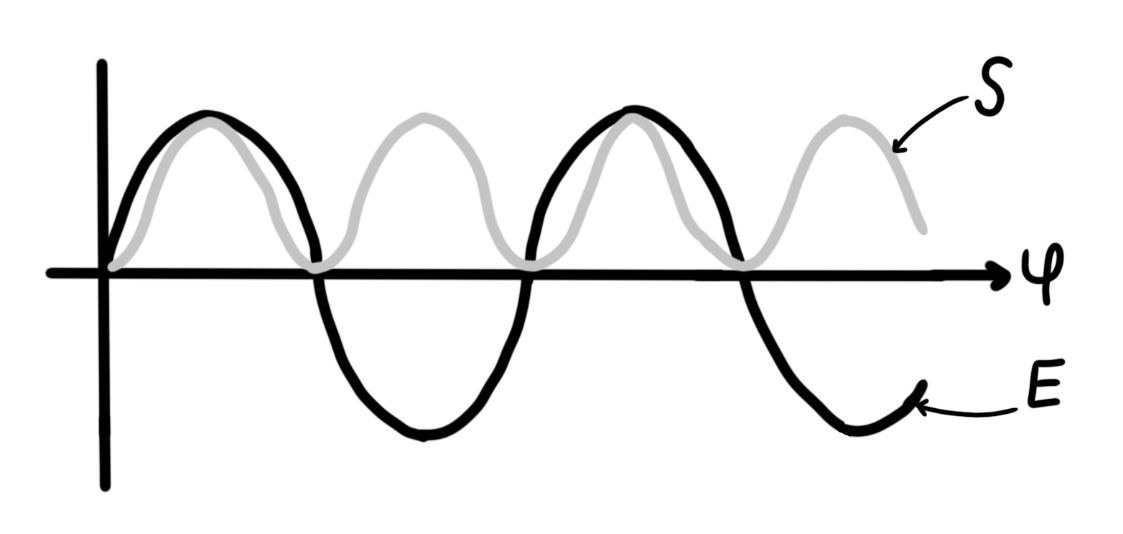
\includegraphics[width=\textwidth]{im/100.png}% Ваше изображение
\end{minipage}%
\hfill
\begin{minipage}[c]{0.6\textwidth} % Правая часть: текст
    \[
    <S>=\frac{c}{8\pi} \sqrt{\frac{\varepsilon}{\mu}} E_0^2
    \]
\end{minipage}

\subsection*{Поляризация}

\[
\begin{aligned}
    \vec{k}
    \quad
    \begin{array}{ll}
        \vec{E}_1=\vec{E}_{01}e^{i\varphi} \\
        \vec{E}_2=\vec{H}_{02}e^{i\varphi}     
    \end{array}
    \quad
    \varphi=\vec{k}\vec{r}-\omega t
\end{aligned}
\]

Как выглядит и как изменяется в пространстве и во времени вектор \( \vec{E}_1+\vec{E}_2 \) ?

\[
\begin{aligned}
    \begin{array}{c|c|c}
    E_{02}=0 & \begin{array}{ll} \vec{E}_{01}=E_{01}\vec{e}_x \\ \vec{E}_{02}=E_{02} \vec{e}_{y} \end{array} & \begin{array}{ll} \vec{E}_{01}=\vec{E}_{01}e^{i\Delta\varphi}e^{i\varphi}  \\ \vec{E}_{02}=\vec{E}_{02}  e^{i\varphi}  \end{array} \\
    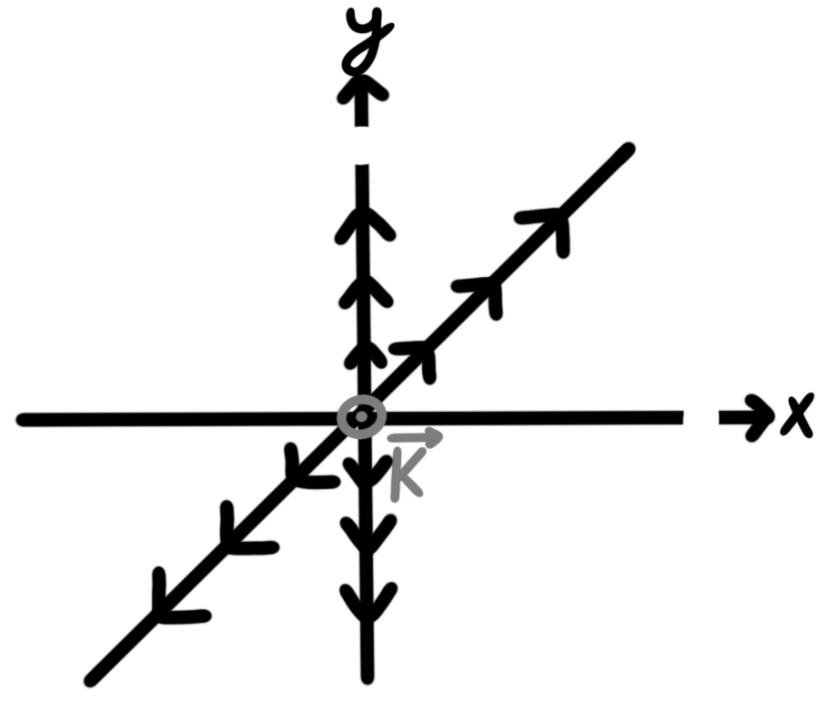
\includegraphics[width=0.2\textwidth]{im/101.png} & 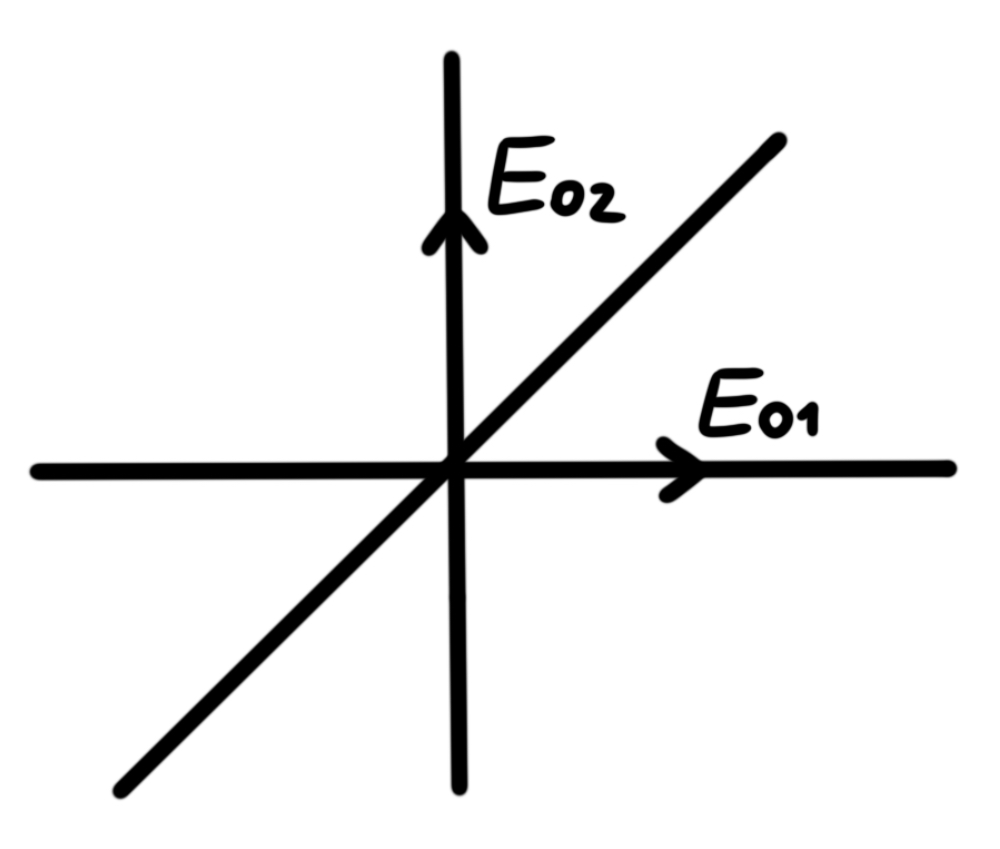
\includegraphics[width=0.2\textwidth]{im/105.png} & 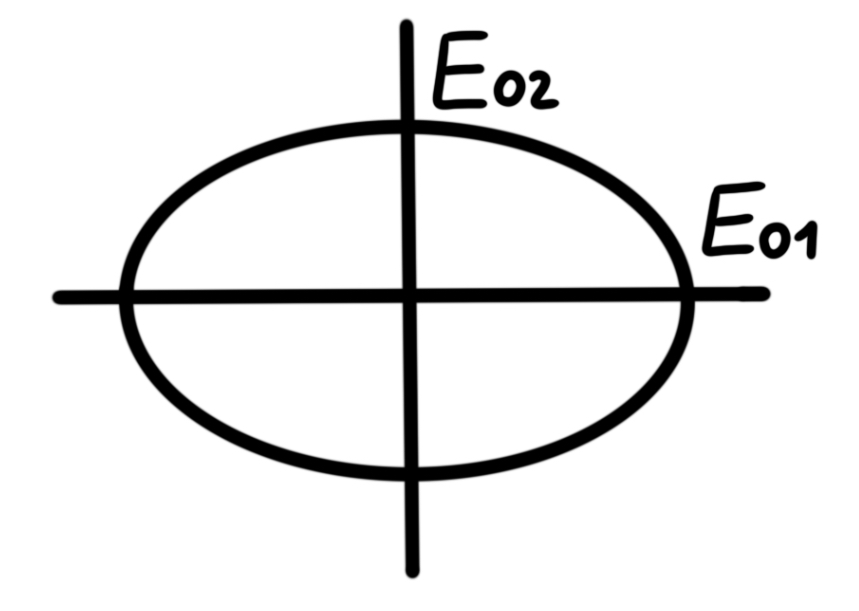
\includegraphics[width=0.2\textwidth]{im/102.png} \\
    \text{Лин.поляриз.} & \text{Лин.поляриз.} & \text{Элипт.поляриз.}
    \end{array}
    \begin{array}{ll}
        \vec{E}_{01}=E_{01}\vec{e}_x \\
        \vec{E}_{02}=E_{02}\vec{e}_{y} \\
        \vec{E}_1=E_{01}\vec{e}_x\sin\varphi \\
        \vec{E}_2=E_{02}\vec{e}_{y}\cos\varphi  
    \end{array}
\end{aligned}
\]

\[
\check{E}: \vec{E}=\vec{e}_xRe\check{E}+\vec{e}_yIm\check{E} 
\]

Продолжим физический смысл комплексной записи:

Линейная поляризация: 
Если \( \vec{E}_0\upuparrows\vec{e}_x \quad \check{E}=E_0\cos\varphi\)

\begin{gather*}
    \vec{E}=\vec{E}_0\cos\varphi\rightarrow\check{E}=E_0\cos\varphi\quad(E_0-\text{комплексное число}, E_0=E_{01}+iE_{02}  ) \\
    \check{E}=\frac{E_0}{2}(e^{i\varphi}+e^{-i\varphi}  ) \\
    \check{E}=E_0e^{i\varphi}\rightarrow \vec{E}=E_0\cos\varphi\vec{e}_x+E_0\sin\varphi\vec{e}_y\leftarrow \underset{\text{(левая)}}{\text{круговая поляризация}} \\ 
    \check{E}=E_0e^{-i\varphi}\rightarrow \vec{E}=E_0\cos\varphi\vec{e}_x-E_0\sin\varphi\vec{e}_y\leftarrow \underset{\text{(правая)}}{\text{круговая поляризация}} \\
    \check{E}=ae^{i\varphi}+be^{-i\varphi}\rightarrow \text{какой поляризации это соответвуют?} \\
    \vec{E}=\vec{e}_x (a+b)\cos\varphi+\vec{e}_y (a-b)\sin\varphi
\end{gather*}

\begin{minipage}[c]{0.2\textwidth} % Левая часть: изображение
    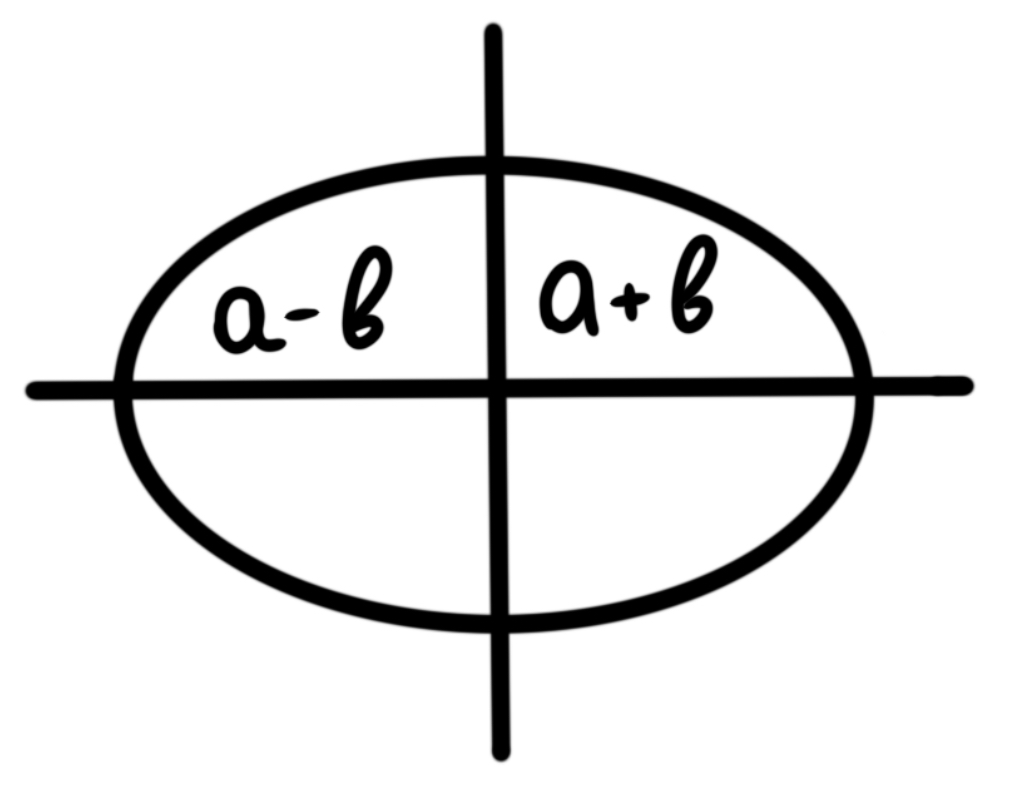
\includegraphics[width=\textwidth]{im/103.png}% Ваше изображение
\end{minipage}%
\hfill
\begin{minipage}[c]{0.6\textwidth} % Правая часть: текст
\[
\check{E}=ae^{i(\varphi-\varphi_0)}+be^{-i(\varphi-\varphi_0)}
\]
\end{minipage}

\begin{minipage}[c]{0.2\textwidth} % Левая часть: изображение
    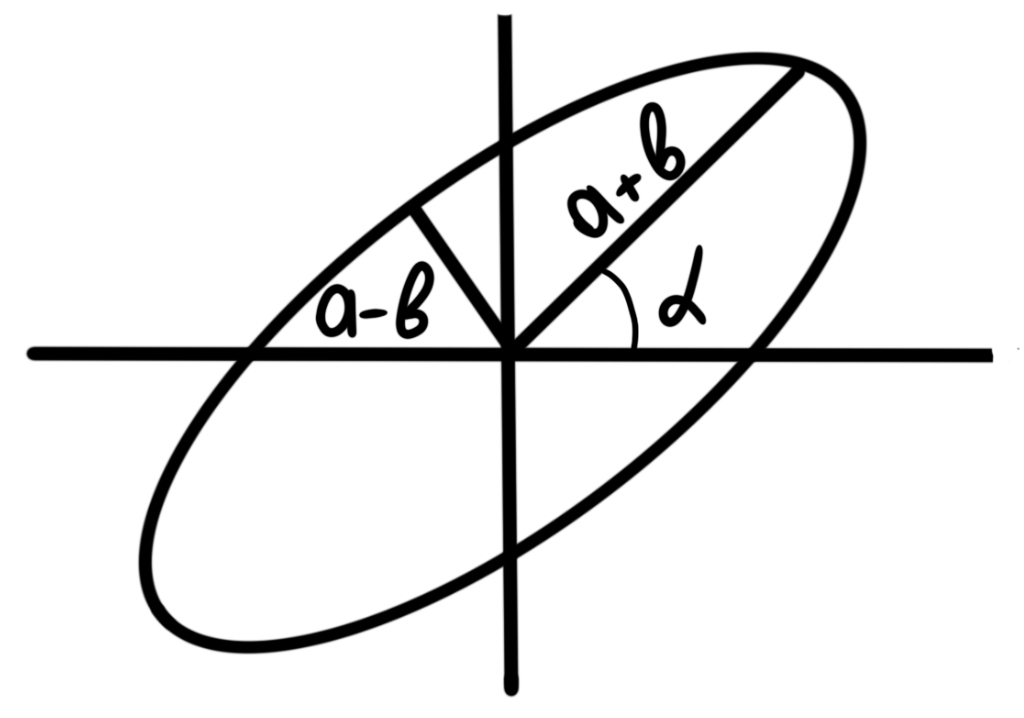
\includegraphics[width=\textwidth]{im/104.png}% Ваше изображение
\end{minipage}%
\hfill
\begin{minipage}[c]{0.6\textwidth} % Правая часть: текст
\[
\check{E}=\left[ae^{i(\varphi-\varphi_0)}+be^{-i(\varphi-\varphi_0)}\right]e^{i\alpha}
\]
\end{minipage}